\section*{Problmea 3}
\subsection*{Problema 3a}
\textbf{Find the minimum value and minimum point of the function \ref{eq:problema4a} on the interval [-1, 1] using the previous implemented algorithms. Compare the results in terms of number of iterations.}
\begin{equation}
    f(x) = -sin(x)+x^2+1
    \label{eq:problema4a}
\end{equation}

La implementación de este problema se encuentra en la carpeta \textcolor{citecolor}{Problema\_3a}. El outut del programa es el siguiente:

\begin{lstlisting}[language=bash]
    Los valores minimos de la funcion son:
	Biseccion:
		Iteraciones	Aproximacion	Tolerancia
			1	0.500000000000	1.000000000000
			2	0.250000000000	0.500000000000
			3	0.375000000000	0.250000000000
			4	0.437500000000	0.125000000000
			5	0.468750000000	0.062500000000
			6	0.453125000000	0.031250000000
			7	0.445312500000	0.015625000000
			8	0.449218750000	0.007812500000
			9	0.451171875000	0.003906250000
			10	0.450195312500	0.001953125000
			11	0.449707031250	0.000976562500
			12	0.449951171875	0.000488281250
			13	0.450073242188	0.000244140625
			14	0.450134277344	0.000122070312
			15	0.450164794922	0.000061035156
			16	0.450180053711	0.000030517578
			17	0.450187683105	0.000015258789
			18	0.450183868408	0.000007629395
			19	0.450181961060	0.000003814697
			20	0.450182914734	0.000001907349
			21	0.450183391571	0.000000953674
			22	0.450183153152	0.000000476837
			23	0.450183033943	0.000000238419
			24	0.450183093548	0.000000119209
			25	0.450183123350	0.000000059605
			26	0.450183108449	0.000000029802
			27	0.450183115900	0.000000014901
			28	0.450183112174	0.000000007451
			29	0.450183110312	0.000000003725
			30	0.450183111243	0.000000001863
			31	0.450183111709	0.000000000931
			32	0.450183111476	0.000000000466
			33	0.450183111359	0.000000000233
			34	0.450183111301	0.000000000116
			35	0.450183111330	0.000000000058
			36	0.450183111345	0.000000000029
			37	0.450183111352	0.000000000015
			38	0.450183111348	0.000000000007
			39	0.450183111347	0.000000000004
			40	0.450183111346	0.000000000002
			41	0.450183111345	0.000000000001
		Solucion: x = 0.450183111345
		Punto de interes: (0.450183111345 , 0.767534424842)
	Newton:
		Iteraciones	Aproximacion	Tolerancia
			1	0.486293632179	0.088517391084
			2	0.450418282152	0.000572696779
			3	0.450183104164	0.000000017319
			4	0.450183111276	0.000000000000
		Solucion: x = 0.450183111276
		Punto de interes: (0.450183111276 , 0.767534424842)
	Secante:
		Iteraciones	Aproximacion	Tolerancia
			1	0.270150596267	2.540301727194
			2	0.524212950303	0.423428390794
			3	0.447630513809	0.182708997709
			4	0.450149038877	0.006212974468
			5	0.450183127397	0.000082970297
			6	0.450183111303	0.000000039191
			7	0.450183111303	0.000000000000
		Solucion: x = 0.450183111303
		Punto de interes: (0.450183111303 , 0.767534424842)
\end{lstlisting}

Comparando estos resultados por las iteracione que tienen que realizar para obtener una respuesta vemos que el método de Newton es el más eficiente de todos, esto se debe que esta basado en un descendiente que se dirige hacia los valores críticos que queremos encontrar. El menos eficiente es el de bisección, esto se debe a que esta basado en una diferencia en los límites del intervalo.

Comparando las soluciones observamos que para el redondeo a 9 decimales las tres tienen la misma solución.

El comando para compilar el programa es el siguiente:

\begin{lstlisting}[language=bash]
    gcc -Wall -Wextra -Werror -pedantic -ansi -o main.out main.c -lm -std=c11
\end{lstlisting}

\subsection*{Problema 3b}
\textbf{Compare and comment the results obtained for each algorithm on the interval [-1, 1] with function \ref{eq:problema4b}.}
\begin{equation}
    f (x) = sin(x) - x^2 + 1
    \label{eq:problema4b}
\end{equation}

La implementación de este problema se encuentra en la carpeta \textcolor{citecolor}{Problema\_3b}. El outut del programa es el siguiente:

\begin{lstlisting}[language=bash]
    Los valores minimos de la funcion son:
	Biseccion:
		Iteraciones	Aproximacion	Tolerancia
			1	0.500000000000	1.000000000000
			2	0.250000000000	0.500000000000
			3	0.375000000000	0.250000000000
			4	0.437500000000	0.125000000000
			5	0.468750000000	0.062500000000
			6	0.453125000000	0.031250000000
			7	0.445312500000	0.015625000000
			8	0.449218750000	0.007812500000
			9	0.451171875000	0.003906250000
			10	0.450195312500	0.001953125000
			11	0.449707031250	0.000976562500
			12	0.449951171875	0.000488281250
			13	0.450073242188	0.000244140625
			14	0.450134277344	0.000122070312
			15	0.450164794922	0.000061035156
			16	0.450180053711	0.000030517578
			17	0.450187683105	0.000015258789
			18	0.450183868408	0.000007629395
			19	0.450181961060	0.000003814697
			20	0.450182914734	0.000001907349
			21	0.450183391571	0.000000953674
			22	0.450183153152	0.000000476837
			23	0.450183033943	0.000000238419
			24	0.450183093548	0.000000119209
			25	0.450183123350	0.000000059605
			26	0.450183108449	0.000000029802
			27	0.450183115900	0.000000014901
			28	0.450183112174	0.000000007451
			29	0.450183110312	0.000000003725
			30	0.450183111243	0.000000001863
			31	0.450183111709	0.000000000931
			32	0.450183111476	0.000000000466
			33	0.450183111359	0.000000000233
			34	0.450183111418	0.000000000116
			35	0.450183111388	0.000000000058
			36	0.450183111374	0.000000000029
			37	0.450183111367	0.000000000015
			38	0.450183111370	0.000000000007
			39	0.450183111368	0.000000000004
			40	0.450183111368	0.000000000002
			41	0.450183111367	0.000000000001
		Solucion: x = 0.450183111367
		Punto de interes: (0.450183111367 , 1.232465575158)
	Newton:
		Iteraciones	Aproximacion	Tolerancia
			1	0.486253486285	0.088418337763
			2	0.450418281731	0.000572695669
			3	0.450183125641	0.000000035083
			4	0.450183111233	0.000000000000
		Solucion: x = 0.450183111233
		Punto de interes: (0.450183111233 , 1.232465575158)
	Secante:
		Iteraciones	Aproximacion	Tolerancia
			1	0.270150596150	2.540301726750
			2	0.524212950377	0.423428391017
			3	0.447630513789	0.182708997931
			4	0.450149038813	0.006212974357
			5	0.450183127333	0.000082970297
			6	0.450183111285	0.000000039080
			7	0.450183111285	0.000000000000
		Solucion: x = 0.450183111285
		Punto de interes: (0.450183111285 , 1.232465575158)
\end{lstlisting}

De igual manera se comprueba que en terminos del número de iteraciones, el método de Newton es el más eficiente y el menos eficiente es el método de bisección. Y las diferencias entre resultados se presenta a partir del añadir más de 9 decimales a la solución.

En la grafica \ref{fig:problema3} se visualizando graficamente la solución del problema 3a y 3b.
\begin{figure}[H]
    \centering
    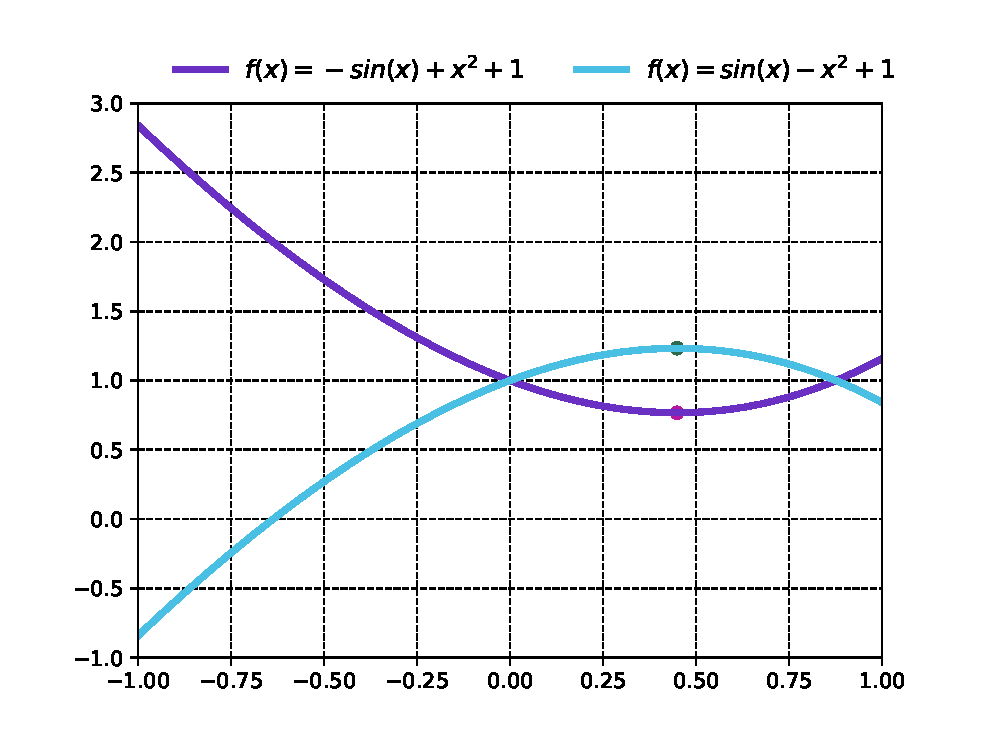
\includegraphics[width=14cm]{Graphics/problem2.eps}
    \caption{Grafica de la función \ref{eq:problema4a} y \ref{eq:problema4b} con su valor mínimo y máximo respectivamente.}
    \label{fig:problema3}
\end{figure}

El comando para compilar el programa es el siguiente:

\begin{lstlisting}[language=bash]
    gcc -Wall -Wextra -Werror -pedantic -ansi -o main.out main.c -lm -std=c11
\end{lstlisting}